\part{Metodologia}

\chapter[Metodologia]{Metodologia}

Este capítulo é destinado à apresentar toda a metodologia aplicada a esta
pesquisa. Vale ressaltar que a metodologia proposta nesta pesquisa está sendo
baseada na definição proposta por Silva e Menezes, que afirmam que toda pesquisa
tem como objetivo encontrar respostas para hipóteses propostas
\cite{da2005metodologia}

Com essa definição em pauta, as hipóteses proposta para a execução deste trabalho neste trabalho foi a seguinte:

\begin{center}
\textit{É possível melhorar a recomendação baseada em conteúdo de pacotes para
usuários de sistemas GNU/Linux levando em consideração o contexto de uso dos pacotes já instalados ?}
\end{center}

Baseado nesta hipótese central, pode-se ver que a pesquisa sendo desevolvida se
enquadra como aplicada, quantitativa, exploratória, bibliográfica e
experimental.


\section{Trabalhos relacionados}

Durante a pesquisa deste trabalho, encontrou-se alguns trabalhos que também estudam recomendação baseada em contexto, sendo o tempo um dos
principais atributos do contexto. Em \cite{lee2008time}, o tempo é usado para gerar avaliação implícita para um histórico de
compras de diversor usuários. Tal abordagem foi comparada com um modelo de recomendação colaborativa tradicional, usando avaliação explícita dos usuários,
sem considerar o tempo. Segundo a pesquisa, percebeu-se um aumento de precisão quando o tempo foi usado para gerar a matriz de recomendação.

Outra pesquida relacionada foi a de \cite{ding2005time}. Nesta pesquisa, um sistema recomendação sensível ao tempo foi criado. o sistema proposto usava uma função de
decaimento exponencial para priorizar itens recentemente avaliados e diminuir o peso de itens avaliados a mais tempo na recomendação. Quando comparado a um sistema de
recomendação colaborativa clássico, percebeu-se um aumento de acurácia para o recomendador sensível ao tempo.

Além de comparação de sistema de recomendação, foi também encontrado um trabalho que propõe um modelo diferente do clássico uso do tempo em recomendação, como o usado em
\cite{ding2005time}. Este modelo foi proposto no artigo de \cite{basile2015modeling}, onde basicamente itens mais antigos não tem seu peso puramente discartado, e sim caso
seu conteúdo seja diferente dos novos itens sendo recomendados. Baseado nos testes realizados, percebeu-se que criar o modelo de usuário dessa formas apresenta vantagens sobre
a forma mais padrão de se usar o tempo para recomendação. Entretanto, o trabalho ainda precisa ser testado em bancos de dados de maior escala para poder aferir melhor seus
resultados

Por fim, um famoso trabalho que usa o contexto de tempo para recomendação se dá na pesquisa \cite{koren2010collaborative}, que apresenta o modelo de recomendação vencedor
do concurso criado pelo Netflix para aumentar a acurácia de suas recomendações de filme. A pesquisa citada usa como diferencial a análise do tempo da avaliação dos filmes
realizados pelos usuários em um modelo similar a pesquisa de \cite{basile2015modeling}


\section{Hipóteses}

Considerando um sistema de recomendação para pacotes usando o tempo como variável de contexto, as seguinte hipóteses foram definidas:

\begin{itemize} \item \textit{\textbf{Ao aumentar o peso de pacotes
recentemente usados no sistema, o perfil do usuário gerado será mais preciso,
ocasionando assim uma recomendação mais apropriada.}} Ao usar o tempo de uso dos
pacotes no sistema, e priorizar os pacotes mais recentemente usados na criação
do perfil de usuário, acredita-se que a mesma irá produzir um perfil mais
consistente do usuário, gerando assim recomendações mais efetivas.\item
\textit{\textbf{Uma abordagem por aprendizado de máquina irá se comportar melhor
        que uma determinística para o problema proposto}}
Considerando os dados presentes em pacote Debian que podem ser
usados para prover a recomendação, pode-se entender que o uso de uma abordagem
por aprendizado de máquina irá prover melhores resultados, devido a possível
complexidade dos relacionamentos entre os atribuitos dos pacotes.
\end{itemize}

\section{Planejamento da pesquisa}

Com o intuito de responder a questão principal do trabalho, juntamente com as
hipóteses propostas, um fluxo de trabalho foi definido. A Figura
\ref{fig:planejamento_pesquisa} sistematiza tal fluxo, facilitando assim a visualização do processo adotado.

\begin{figure}[h]
  \centering
  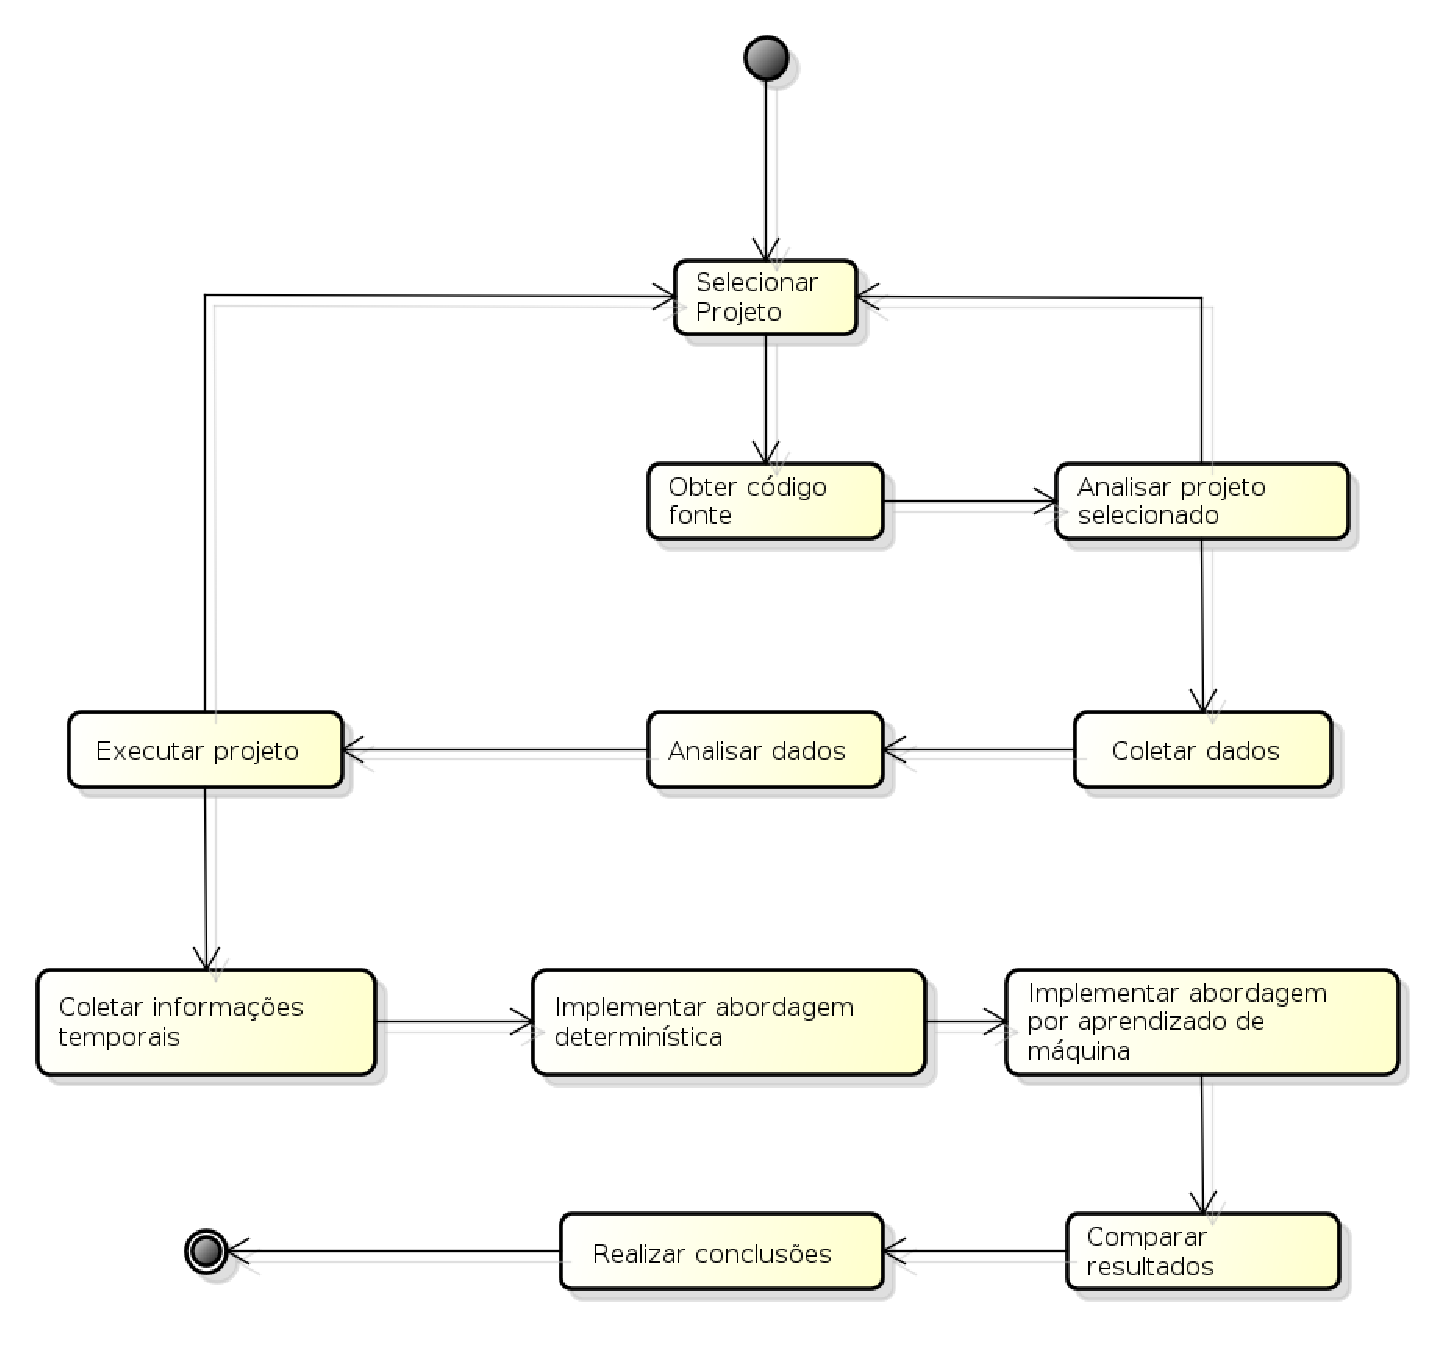
\includegraphics[width=0.9\textwidth]{figuras/planejamento_pesquisa.eps}
  \caption{Processo usando para realização das atividades dessa pesquisa}
  \label{fig:planejamento_pesquisa}
\end{figure}

\begin{enumerate}

    \item \textbf{Selecionar projeto:}
Selecionar um projeto de software livre que implemente um sistema de recomendação baseada em conteúdo e que não leve em consideração questões temporais do pacote quando se realiza tanto
a criação do perfil de usuário e a recomendação propriamente dita. Além disso, deve-se também levar em consideração as dependências do projeto, desde os bibliotecas que depende e os
dados necessitados. Caso o projeto necessite de dados que não possam ser obtidos pelo pesquisadores deste trabalho, o mesmo não poderá ser considerado.

    \item \textbf{Obter código fonte:}
Obter o código fonte do projeto em questão, para que o mesmo possa ser alterado visando o estudo das hipóteses levantadas

    \item \textbf{Analisar projeto selecionado:}
Nesta etapa, o projeto deve ser analisado, visando a compreensão de como o mesmo funciona e, principalmente, os dados necessários para a execução adequada do projeto.

    \item \textbf{Coletar dados:}
Para prover os possíveis dados necessários para o projeto selecionado, uma estratégia de coleta de dados precisa ser definida e implementada.

    \item \textbf{Análisar dados:}
Será necessário analisar os dados coletados, visando descartar dados inválidos e classificar o que foi coletado conforme as necessidades do projeto escolhido.

    \item \textbf{Executar projeto selecionado:}
Com os dados e as dependências do projeto resolvidas, o mesmo deve ser executado, visando encontrar possíveis problemas de execução que não foram previstos e também observar as funcionalidades do projeto.

    \item \textbf{Coletar informações temporais:}
Deve-se implementar uma forma de coletar as informações temporais dos pacotes sendo usados pelo usuário e também prover uma forma de classificar essa informação coletada.

    \item \textbf{Implementar abordagem deterministica:}
Para responder a primeira questão proposta, será necessária implementar uma equação matemática que use as informações de tempo coletadas, juntamente com os outros atributos já usados no projeto selecionado para prover um recomendação.

    \item \textbf{Implementar abordagem por aprendizado de máquina:}
Implementar uma abordagem não-deterministica, no caso uma estratégia de aprendizado de máquina, para usar as informações de tempo coletadas juntamente com os outros atributos providos pelo projeto selecionado para compor um a recomendação.

    \item \textbf{Comparar resultados:}
Para responder as hipóteses propostas será necessário não só comporar as duas abordagens propostas, determinística e não determinística, e sim comparar ambas também com as abordagens já implementadas pelo projeto proposto e verificar se as hipótes se sustetam.

    \item \textbf{Realizar conclusões:}
Com a comparações de resultados feita, a mesma deve ser analisada e conclusões devem ser geradas baseada nos fatos apresentados.
\end{enumerate}


\section{Teste de hipótese}

O projeto selecionado para testar as hipóteses foi o \textit{AppRecommender}, o recomendador de pacotes para distribuições Debian que implementa tanto estratégias de recomendação por conteúdo quanto colaborativas \cite{araujo2011apprecommender}.
Apesar do AppRecommender usar questões temporarais providas pelo pacote popularity-contest nas suas recomendações, tal atributo temporal só é explorado nas recomendações colaborativas, e não nas baseadas em conteúdo, fazendo com que o projeto passe no critério de seleção estabelecido.

\begin{description}

\item[Obtenção do código fonte]

O código fonte da aplicação AppRecommender pode ser encontrada no repositório de projetos Github \footnote{\url{https://github.com/tassia/AppRecommender}}.
Vale ressaltar que as modificações realizadas foram realizadas em uma cópia local do mesmo, sendo essa mantida pelos pesquisadores deste trabalho.

\item[Analisar projeto selecionado]

Um vez obtido o código fonte do projeto, identificou-se algumas questõs
importantes. A primeira delas foi que algumas bibliotecas não estavam mais
presentes no repositório de pacotes de versões mais recentes do Debian, no caso,
o Debian jessie. A segunda problemática foi relacionada a obtenção do dados.
Mediante uma análise tanto do ponto de vista de recomendação tanto do ponto de
vista dos experimentos de validação usados para avaliar os algoritmos
desenvolvidos, percebeu-se diversos e distintos conjuntos de dados necessários.
A Tabela \ref{tab:dados_apprecommender} mostra os dados necessários e o contexto
onde são usados:
\end{description}


\section{Dados}

Para o projeto selecionado, a análise realizada pode ser vista na Tabela
\ref{tab:dados_apprecommender}. Tal tabela mostra os dados usados no
AppRecommender e como os mesmos podem ser obtidos.

\begin{table}[h]
\centering
\resizebox{\textwidth}{!}{\begin{tabular}{|l|l|l|l|}
\hline
\rowcolor[HTML]{EFEFEF}
{\textbf{Dados}} & {\textbf{Contexto}} & {\textbf{Coleta}} \\ \hline
Lista de pacotes válidos &
\parbox{10cm}{Esta lista irá ser usada na criação de uma índice de busca Xapian,
que será usado para realizar a recomendação} &
\parbox{10cm}{Pode-se usar os scripts get\_axipkgs.py obter todos os possíveis
pacotes Debian,ou usar o srcipt get\_programs.sh, que irá selecionar
só pacotes que contém a Debtag role:;program, indicando que o mesmo é um
pacote executável.}\\ \hline
Índice xapian de pacotes do usuário &
\parbox{10cm}{Usado tanto para estratégias de recomendação por conteúdo,
 colaborativas e híbridas}&
\parbox{10cm}{Este Índice pode ser gerado via execução do script indexer\_axi.py
 passando os parâmetros certos}\\ \hline
Debtags válidas&
\parbox{10cm}{Usado para filtrar os pacote que serão usados na
recomendação}&
\parbox{10cm}{Pode ser obtido pelo script get\_tags.py}\\ \hline
Submissões do popularity contest&
\parbox{10cm}{Usada para criar um índice Xapian de submissões do
popularity-contest}&
\parbox{10cm}{O projeto não provê uma forma automatizada de coletar tais dados,
devido ao fato do mantenedor do projeto não fornecer tais dados.}\\ \hline
Indíce Xapian para submissões do popularity contest &
\parbox{10cm}{Usado tanto para a realização de recomendações colaborativas e
híbridas, assim como para a execução dos experimentos usados
para avaliar as soluções desenvolvidas.} &
\parbox{10cm}{Pode ser obtido pela execução do script indexer\_popcon.py.
Entretanto, vale ressaltar que esse script parte do princípio que já existem
submissões do popularity contest coletadas previamente.}\\ \hline
\end{tabular}}
\caption{Dados necessários para execução do AppRecommender}
\label{tab:dados_apprecommender}
\end{table}

Conforme pode ser observado na Tabela \ref{tab:dados_apprecommender}, muito dos dados
necessários para a execução do AppRecommender podem ser obtidos de forma automatizada
por scripts de coleta. Entretanto, este não é o caso para as submissões do
popularity contest. Isso se dá pelo fato da aplicação não disponibilizar as submissões
propriamente ditas, e sim as análises estatísticas feitas em cima das mesmas. Para o
AppRecommender, tais dados foram obtidos por intermédio de um Debian Developer, sendo
que algumas questões de relacionada a privacidade dos usuários se tornou necessária.
\cite{araujo2011apprecommender}. Tal problemática dificulta bastante o uso das
estratégias colaborativas do AppRecommender, pois dependem desse banco de dados
de submissões do popularity-contest. Entretanto, foi levantado também que os
experimentos de comparação entre os algoritmos implementados também dependem
desses dados, porém em menor escala do que uma recomendação colaborativa.
Dessa forma, foi necessário pensar em uma estratégia
de coleta de dados, principalmente visando o funcionamento dos experimentos propostos
para a avaliação dos algoritmos.

\section{Engenharia de Atributos}

Considerando as limitações da obtenção de dados já discutidas, a pesquisa teve
como objetivo então se focar na recomendação baseada em conteúdo. Dessa forma,
vale a pena detalhar os dados usados para fazer essa recomendação.

Considerando que apenas pacotes Debian podem ser recomendados, os dados sendo
usados atualmente para a realização de uma recomendação podem ser vistos no
arquivo \textit{control} encontrado em qualquer pacote Debian, conforme pode ser
visto na Figura \ref{fig:control_pacote}

\begin{figure}[h]
  \centering
  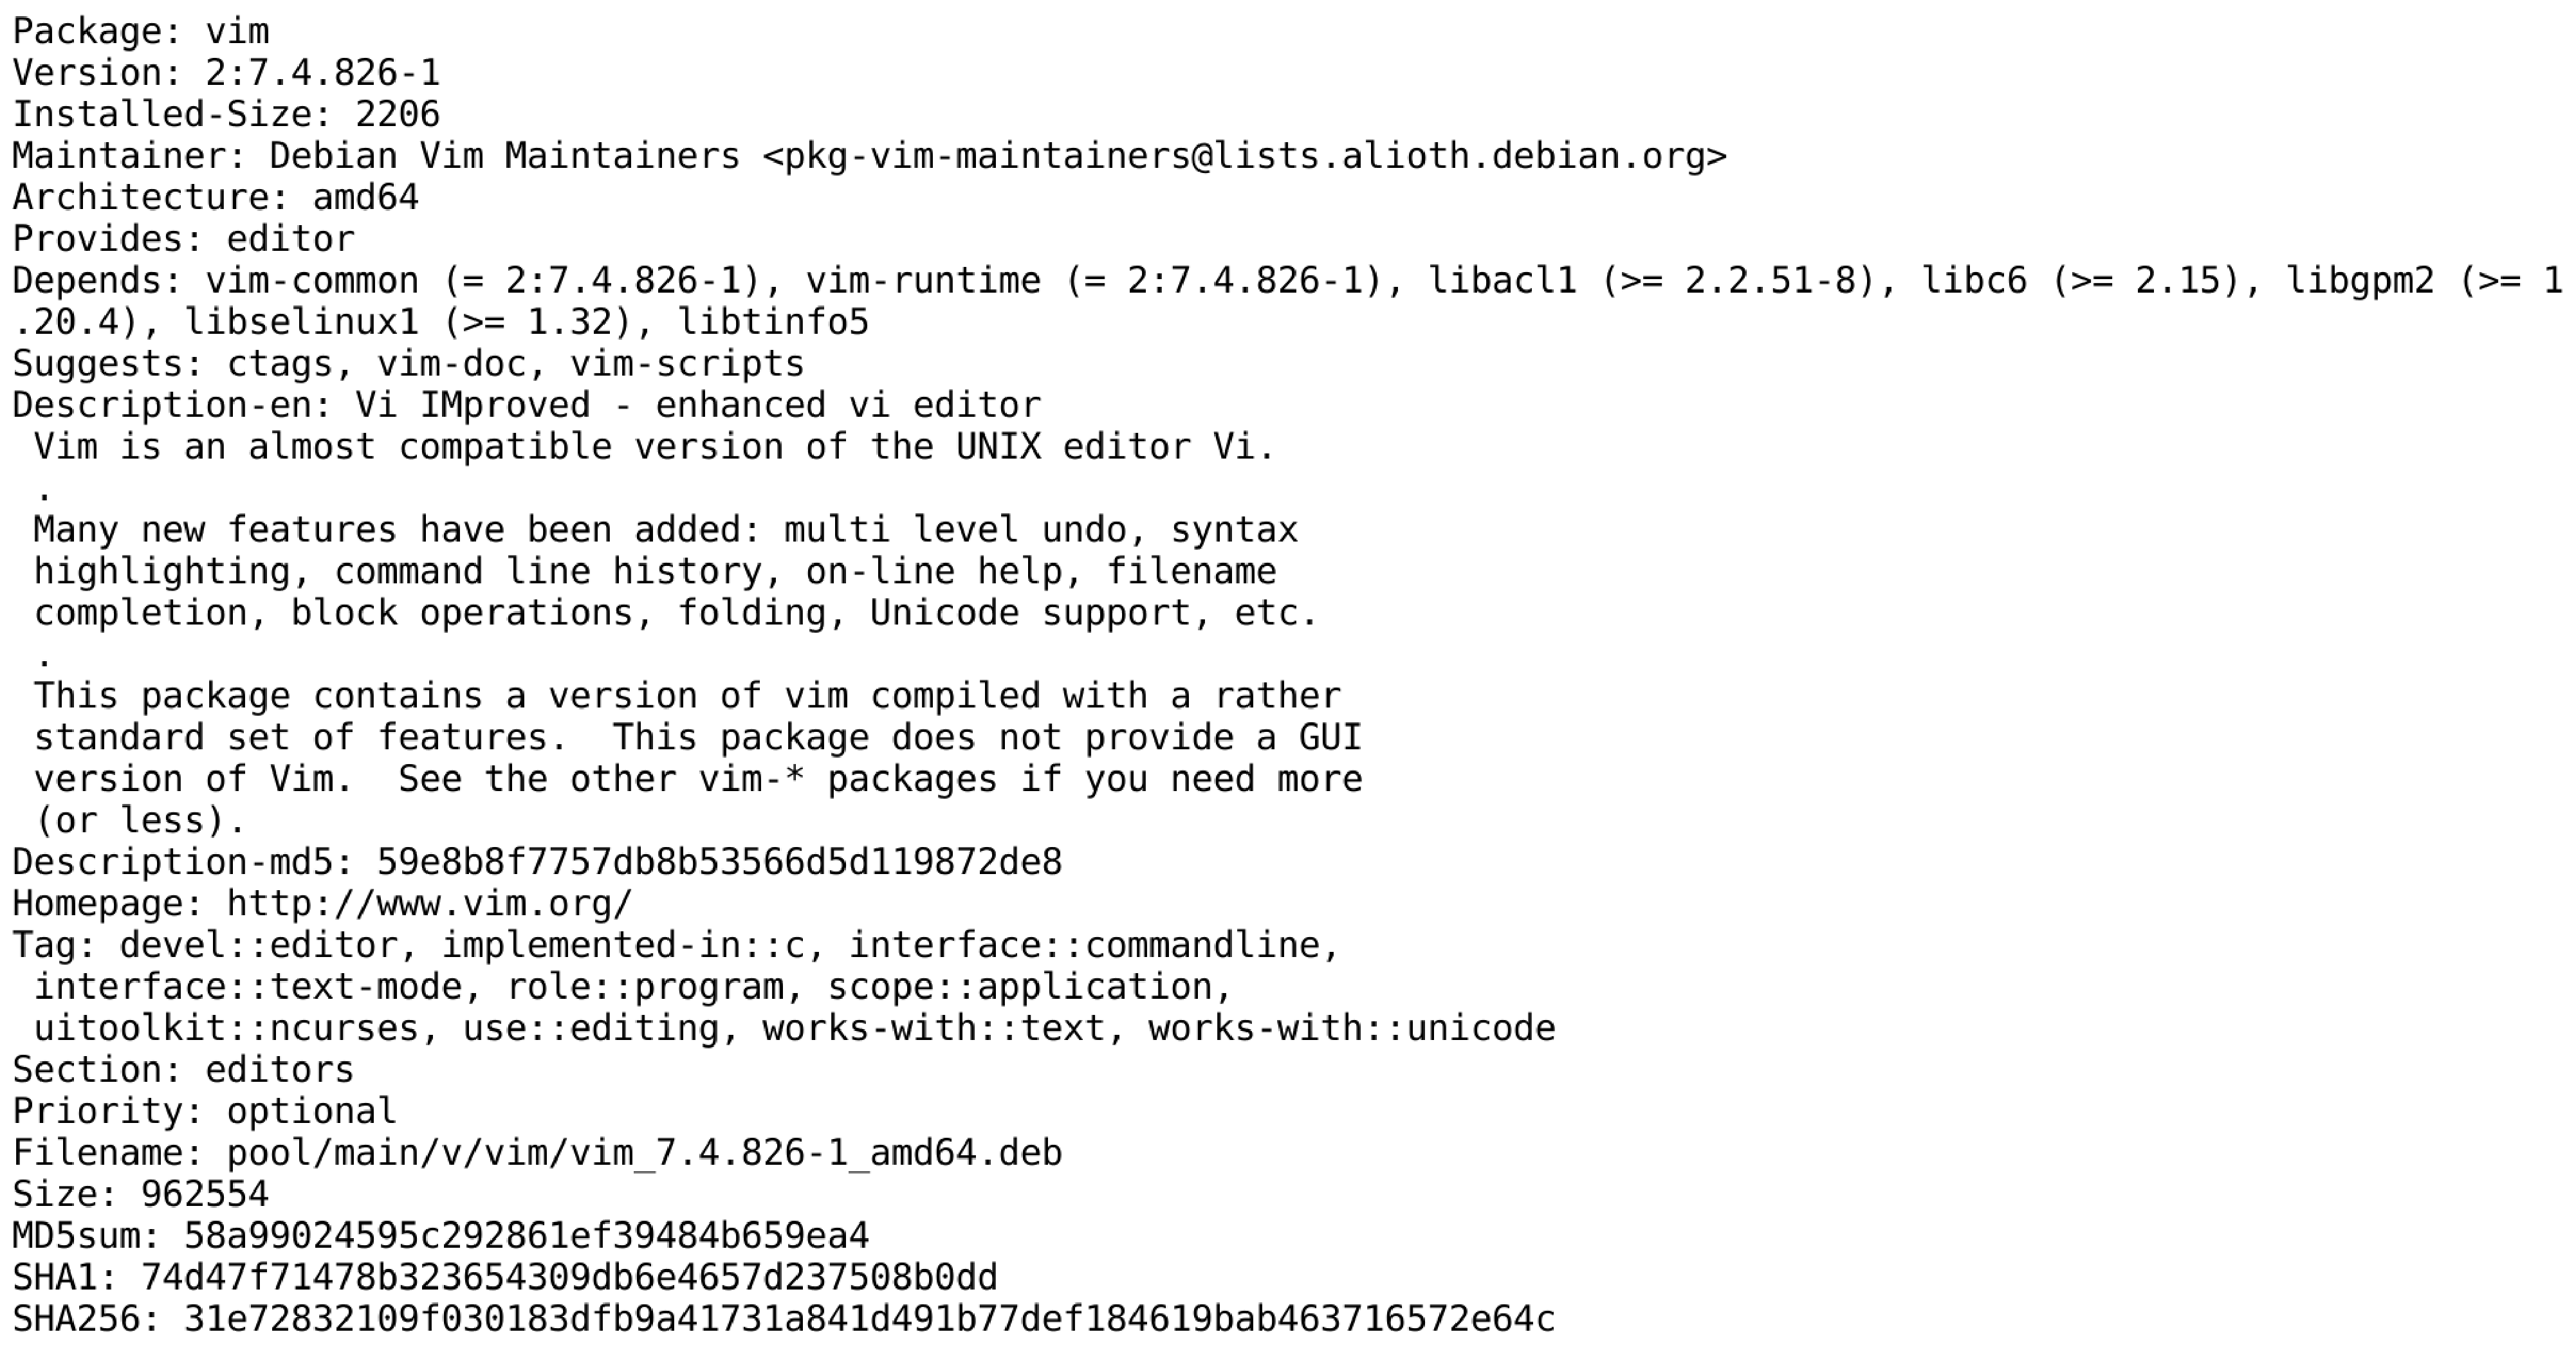
\includegraphics[width=0.9\textwidth]{figuras/control_pacote.eps}
  \caption{Arquivo control de um pacote Debian}
  \label{fig:control_pacote}
\end{figure}

Pode-se ver na Figura \ref{fig:control_pacote} os principais dados usados na
recomendação de um pacote, sendo eles as debtags e a descrição dos pacotes.

As debtags são basicamente um forma de melhor categorizar um pacote fora das 33
seções disponíveis no Debian, além também de permitir que um pacote seja
categorizado em diferentes frentes ao mesmo tempo \cite{zini2005cute}. Isso pode ser visto na Figura
\ref{fig:control_pacote}, onde o software \textit{vim} possui as debtags
\textit{devel::editor} e \textit{interface::commandline}, ou seja, está se
enquadrando tanto como um editor de texto e uma aplicação que roda em linha de
comando.

O processo de criação de debtags é manual, ou seja, um usuário deve associar uma
debtag a um pacote e a comunidade Debian deve verificar se aquela debtag
sugerida condiz com a aplicação em si. Atualmente, existem X pacotes
categorizados com debtags.

Por fim, vale lembrar que nem todas as debtags são consideradas significativas
para o processo de recomendação, sendo que uma filtragem é realizada visando
selecionar apenas as debtags válidas para a construção do perfil do usuário.

A segunda fonte de dado usada é a descrição do pacote, sendo no caso cada termo
individual. A descrição de um pacote é realizada pelo empacotador na hora com
que o mesmo cria o arquivo \textit{control}.

Com essas duas informações, o AppRecommender cria então um perfil de usuário
onde os termos de maior peso são usados para compor tal perfil. Isso é feito por
algoritmos como \textit{Term Frequency Inverse Document Frequency Sub-Linear}
(TFIDF-sublinear) e \textit{Expansão de Query} (ESet).

O perfil de usuário criado é então usado para consultar toda a base de pacotes
do Debian. Isso é realizado através do \textit{apt-xapian-index}, uma aplicação
que provê uma forma de busca pacotes no Debian por meio de Queries, sendo que no
caso do AppRecommender, a query de busca é o perfil gerado para o usuários.
Finalmente, os pacotes retornados são então a recomendação final da aplicação.

Dado esse conjunto de dados, o novo atributo que esta pesquisa pretende
adicionar é o contexto de uso de um pacote, sendo no caso, a última vez que o
mesmo foi usado. Em distribuições Debian, isso pode ser verificado via comando
\textit{stat} o binário do pacote, que tem uma saída que pode ser visualizada na Figura
\ref{fig:comando_stat}.

\begin{figure}[h]
  \centering
  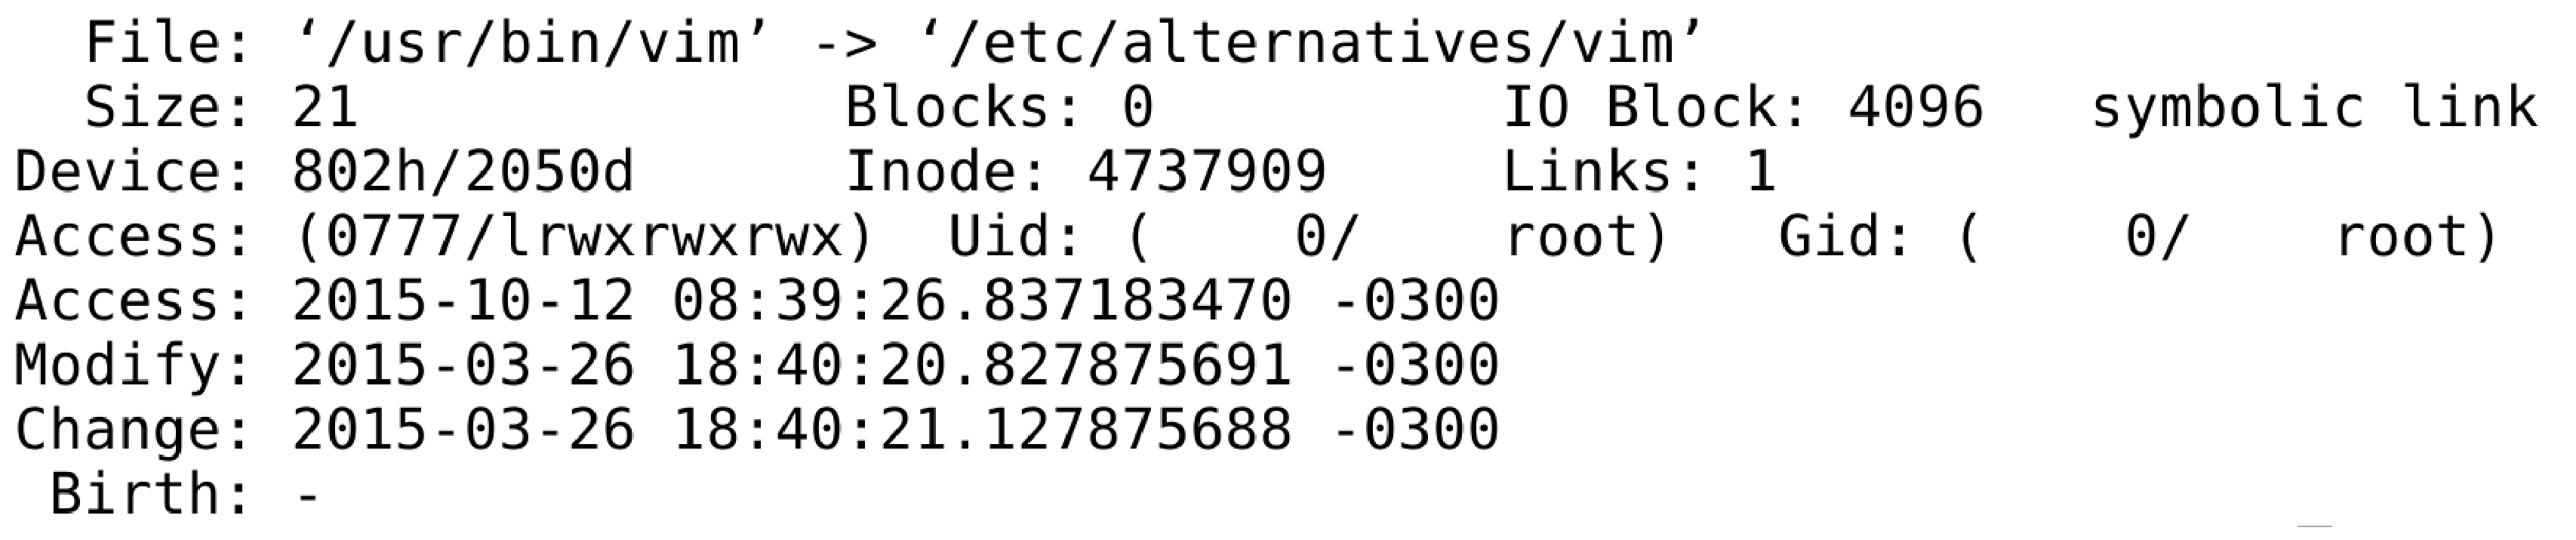
\includegraphics[width=0.9\textwidth]{figuras/comando_stat.eps}
  \caption{Saída do comando \textit{stat} para um dado software}
  \label{fig:comando_stat}
\end{figure}

Pode ser visto na Figura \ref{fig:comando_stat} que o comando exibe os seguintes
atributos de tempo de um dado arquivo \cite{1_haas}:

\begin{itemize}
    \item \textbf{Access:} Última vez que um arquivo foi acessado, ou seja, a
        última vez que seu conteúdo foi de fato acessado.
    \item \textbf{Modify:} Última vez que conteúdo de um arquivo foi modificado.
    \item \textbf{Change:} Última vez que o status de um arquivo foi modificado,
        como mudar as permissões do arquivo e o seu done, ou seja, modificar o
        inode do arquivo.
\end{itemize}

Dessa forma, pode ser visto que o campo \textit{Access} de um arquivo é um dos
principais indicadores de uso de um pacote. Entretanto, o Debian apresenta uma
restrição neste campo. Isso acontece devido a como o sistema de arquivos é
configurado,

pois algumas flags especiais podem ser usadas para alterar como
esse campo é preenchido \cite{2_wiki.debian.org}:

\begin{itemize}
    \item \textbf{noatime:} O sistema de arquivos não irá computar o tempo de
        acesso do arquivo.
    \item \textbf{stricatime:} O sistema de arquivos irá sempre alterar o tempo
        de acesso do arquivo.
    \item \textbf{relatime:} O sistema de arquivos só irá computar o tempo de
        acesso de um arquivo se o valor desse campo for menor que os valores dos
        campos \textit{Modify} e \textit{Change}. Esse opção é default desde
        o kernel 2.6.30, e além disso uma adição foi feita, o tempo de acesso será
        modificado se o mesmo for mais antigo que um dia.
\end{itemize}

O uso do relatime passou a ser default para montar o sistema de arquivos devido
aos problemas de perfomance ocasionados pelo atime. Segundo Ingo Molnar, "atualizar o valor
de atime é de longe uma das deficiências de performance que o Linux possuir
hoje" \cite{3_corbet_2007}. Sendo assim, as informações de contexto que serão
usadas, tempo de acesso, modificação e mudança, são aproximações e assim não
refletem perfeitamente o contexto de uso dos pacotes.

Sendo assim, a informação temporal de cada pacote será obtida pela seguinte
fórmula:

ClassificaçãoTempo = $\frac{TempoAcesso - TempoModificação}{TempoAtual -
TempoModificação}$


Onde:

\begin{itemize}
    \item \textbf{TempoAcesso:} Tempo de último acesso do pacote em segundos.
    \item \textbf{TempoModificação:} Tempo de última modificação do pacote em
        segundos.
    \item \textbf{TempoAtual:} Tempo atual no qual o usuário executa a
        aplicação em segundos.
\end{itemize}


A equação apresentada irá retornar um valor de 0 a 100, sendo que quanto mais
perto de 100, mais recente é considerado o arquivo. Vale ressaltar que a fórmula
também leva em conta o tempo de modificação, pois em algumas situações alterar o
tempo de modificação também altera o tempo de acesso, podendo ocasionar que um
pacote recentemente atualizado tenha um peso maior, mesmo que o usuário não
tenha diretamente o executado.

Vale ressaltar que existe uma limitação quanto a pacotes indiretamente usados,
como por exemplo linguagens de programação. Se um pacote precisar delas para
executar qualquer uma de suas funcionalidades, o tempo de acesso das mesmas
também será atualizado, mesmo que o usuário não tenha diretamente executado o
pacote.


\section{Abordagem determinística}

A proposta da abordagem determinística é criar o perfil de usuário através
dos pacotes instalados que possuem uma maior relevância para o usuário,
essa relevância é determinada utilizando informações de tempo quanto a
utilização do pacote, segue uma imagem contendo o fluxo para realizar uma
recomendação utilzando a abordagem determinística.

\begin{figure}[h]
  \centering
  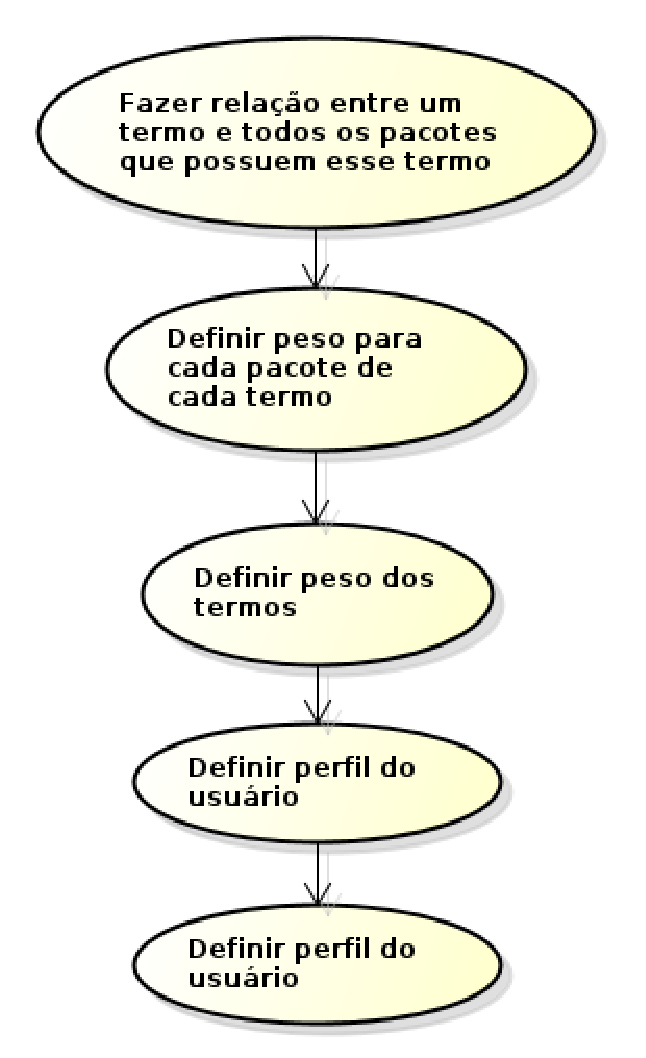
\includegraphics[width=0.9\textwidth]{figuras/abordagem_deterministica.eps}
  \caption{Processo usando para realizar a abordagem deterministica}
  \label{fig:abordatem_deterministica}
\end{figure}

Afim de relacionar um termo, que pode ser uma debtag ou uma descrição, com
os pacotes que o utilizam, sendo esses pacotes todos os pacotes que estão
na base de dados para serem recomendados, é utilizado um dicionário, onde
a chave é o nome do termo, e o valor no dicionário é uma lista com todos os
pacotes que utilizam aquele termo, assim é mantido a relação entre um termo
e todos os pacotes que o utilizam.

Para se calcular o peso de um pacote, primeiramente é atribuído um valor de
0 a 1 ao pacote através de uma função, onde os dados para essa função são:

\begin{itemize}
  \item \textit{\textbf{Tempo de Acesso:}} Tempo do último acesso ao pacote;
  \item \textit{\textbf{Tempo de Modificação:}} Tempo da última modificação do pacote;
  \item \textit{\textbf{Tempo Atual:}} Tempo atual no qual o usuário executa a aplicação.
\end{itemize}

Utilizando esses dados é utilizado a seguinte função, que converte essa
informação de entrada em um peso inicial do pacote, que será a classificação
no tempo do pacote:

\textbf{ClassificaçãoTempo} = $\frac{TempoAcesso - TempoModificação}{TempoAtual -
TempoModificação}$

Afim de atribuir mais peso para pacotes que foram recentemente usados é
utilizado a seguinte função:

\textbf{PesoPacote} = C / $\exp\left(({1 - ClassificaçãoTempo}) * {Alfa}\right)$

Onde C e alfa são constantes definidas através de testes realizados na
aplicação, e os valores achados que mais otimizaram foram:

\textbf{C} = 1

\textbf{Alfa} = 1

Após calcular o peso de cada pacote do termo, o peso to termo é obtido
através da média aritmética dos pesos dos pacotes multiplicado pelo TFIDF,
técnica que já era utilizada no AppRecommender, porém é uma técnica que
também prioriza os termos pela quantidade do termo dividido pela quantidade
total de termos \cite{araujo2011apprecommender}, ou seja:

\textbf{TF\_IDF} = $\frac{QuantidadeDoTermo} {QuantidadeTotalDeTermos}$

\textbf{PesoFuncaoDeterministica} = $\sum_{i=1}^{n} Termo(i)$

\textbf{PesoTermo} = PesoFuncaoDeterministica * TF\_IDF

Utilizar dessa técnica de multiplicar o peso gerado pela função
determinística, que atribui o peso ao termo utilizando a relação entre os
pacotes que utilizam o termo e o tempo de utilização desses pacotes, com
o TFIDF é que a técnica do TFIDF já foi utilizada no AppRecommender, e na
tese da Tássia Camoes, é a técnica mais importante da recomendação de
conteúdo, logo optou-se por levá-la em consideração afim de otimizar os
resultados da recomendação.

Com os pesos de cada termo o perfil do usuário é formado pelos termos com
os maiores pesos, utilizando esse perfil é realizado uma consulta que
retorna os pacotes que possuem maior relevância para o perfil que foi
gerado \cite{araujo2011apprecommender}.


\section{Aprendizado de máquina}

Para a abordagem por aprendizado de máquina, escolheu-se aplicar a
metodologia de filtragem pós-recomendação. Para a projeto em mãos, isso
significa que o mesmo irá continuar fazendo a recomendação conforme foi
desenhado, mas as recomendações serão filtradas pelo perfil de usuário
construído pela abordagem de aprendizado de máquina.

Sendo assim, o enfoque dessa abordagem é usar um algoritmo supervisionado
para criar o perfil do usuário baseado em seus pacotes. Dessa forma, é
necessário definir como cada pacote será apresentado para algoritmo, além de
definir também o valor de cada pacotes.

Para o valor do pacote, definiu-se a seguinte escala de classificação baseada na
fórmula proposta na seção de Engenharia de Atributos:

\begin{table}[h]
\centering
\begin{tabular}{cc}
\hline
\rowcolor[HTML]{EFEFEF}
{Escala} & {Valores} \\ \hline
{Excelent(EX)}  & ClassificaçãoTempo >= 80                  \\ \hline
{Great(G)}   & ClassificaçãoTempo >= 70                  \\ \hline
{Medium(M)}   & ClassificaçãoTempo >= 50                  \\ \hline
{Bad(B)}   & ClassificaçãoTempo >= 30                  \\ \hline
{Horrible(H)}   &ClassificaçãoTempo<30                   \\ \hline
\end{tabular}
\caption{Escala para classificação de um pacote baseado em seus atributos de tempo}
\label{tab:cwe476-erros}
\end{table}


Com a escala definida e as informações de tempo coletadas para cada pacote,
pode-se então criar a classificação de cada pacote manualmente instalado pelo usuário.
Isso se dá tudo por um script automatizado \footnote{\url{https://github.com/TCC-AppRecommender/AppRecommender/tree/master/src/bin}}
que irá realizar tal função.

Uma vez classificados, os pacotes então podem ser usados como entrada para o algoritmo supervisionado.
Entretanto, ainda é necessário definir como os dados presentes no pacote serão usados de entrada para o
algoritmo de aprendizado supervisionado. Considerando que os principais dados do pacote sendo usados na
recomendação são as debtags e as palavras que compõem sua descrição, escolheu-se usar uma abordagem de
vetor binário para cada um dos items. Sendo assim, os vetor de entrada será composto pela agregação de dois vetores
binários.

Para as debtags, o vetor binário irá ter o tamanho igual ao número de debtags definidas pelo Debian. Sendo assim, o
vetor binário irá representar as debtags ordenadas em ordem alfabética. Dessa forma,
o vetor binário de um dado pacote irá conter o valor "0" caso o mesmo não contenha uma debtag e "1" caso a mesma se encontre
no pacote. Por exemplo, dado um conjunto de três debtags role:program, implemented-in:c e devel:editor, e um pacote com a debtag
role:program associado a ele, o seu vetor binário seria o seguinte: [0, 0, 1].

Para os termos da descrição, a formatação do vetor é um pouco diferente. Primeiramente, optou-se por usar os termos apenas presentes
nos pacotes manualmente instalados do usuário e não no banco de dados do Debian. Isso se dá para reduzir o tamanho do vetor e também
pelo fato de que se um termo não aparece em nenhum pacote instalado pelo usuário, o mesmo em tese não terá nenhum peso relevante na
classificação. Além disso, foi necessário retirar termos comuns do vetor de termos produzido, como por exemplo os termos "a" e "the" que
aparecem em praticamente todo pacote mas não representam nenhuma vantagem na hora de avaliar um pacote. Uma vez gerado o vetor de todos os
termos dos pacotes do usuário e aplicar o filtro de termos comuns, a abordagem de vetor binário pode ser usada, funcionando de forma
similar ao vetor binário das debtags, onde os termos estarão representados em ordem alfabética e caso o pacote contenha tal termo em sua
descrição, a posição do vetor associado ao termo será marcada como "1".

Com a combinação desses valores, chega-se então a forma final da forma de entrada de um pacote para o uso de algoritmos de aprendizado
supervisionados. Observa-se também que para propósitos de  armazenamento, a classificação do pacote também é armazenada ao final da combinação
dos vetores binários dos termos e debtags. A Figura X mostra a versão final da formatação de dados de um pacote:

Por fim, os pacotes então podem finalmente ser usados para alimentar o algoritmo de aprendizado escolhido para a pesquisa, sendo no caso um
classificador bayesiano. A escolha desse classe de algoritmo se deu por alguns fatores. O primeiro se dá pela popularidade do algoritmo para
sistemas de recomendação por conteúdo \cite{amatriain2011data}. Outro fator que levou a escolha desse algoritmo é a sua capacidade de produzir
modelos eficazes mesmo quando o número de dados de treinamento não são encontrados em abundância \cite{segaran2007programming}. Essa implicação
quanto aos dados foi feita mediante uma análise do número de pacotes médios para dados usuários, levantamento também realizado por \cite{araujo2011apprecommender}.

Vale ressaltar também que algoritmos de aprendizado supervisionados não-lineares foram considerados, como redes neurais. Entretanto, segundo
a pesquisa realizada por \cite{pazzani1997learning} o uso de redes neurais em relação ao classificador bayesiano não mostra nenhuma melhoria
considerável para sistema de recomendação. Sendo assim, optou-se por usar o classificador bayesiano de início e caso o modelo não apresente
resultados satisfatórios, mudar então para um algoritmo supervisionado não-linear.

É importante também ressaltar que o algoritmo será validado não só pela técnicas usadas no AppRecommender, mas também técnicas próprias de
aprendizado de máquina serão usadas para verificar se o modelo gerado está satisfatório, como a validação cruzada, sendo o foco principal a
identificação de \textit{overfitting} e \textit{underfitting}.

Com o perfil de usuário criado e validado, toda vez que uma recomendação for gerada, os pacotes escolhidos serão filtrados pelo perfil criado,
sendo que apenas os pacotes classificados com EX ou G qualificados para a recomendação ao usuário.


\subsection{Numeração de Páginas}

A contagem sequencial para a numeração de páginas começa a partir da
primeira folha do trabalho que é a Folha de Rosto, contudo a numeração em
si só deve ser iniciada a partir da primeira folha dos elementos textuais.
Assim, as páginas dos elementos pré-textuais contam, mas não são numeradas
e os números de página aparecem a partir da primeira folha dos elementos
textuais que é a Introdução.

Os números devem estar em algarismos arábicos (fonte Times ou Arial 10) no
canto superior direito da folha, a 02 cm da borda superior, sem traços,
pontos ou parênteses.

A paginação de Apêndices e Anexos deve ser contínua, dando seguimento ao
texto principal.

\subsection{Espaços e alinhamento}

Para a monografia de TCC 01 e 02 o espaço entrelinhas do corpo do texto
deve ser de 1,5 cm, exceto RESUMO, CITAÇÔES de mais de três linhas, NOTAS
de rodapé, LEGENDAS e REFERÊNCIAS que devem possuir espaçamento simples.
Ainda, ao se iniciar a primeira linha de cada novo parágrafo se deve
tabular a distância de 1,25 cm da margem esquerda.

Quanto aos títulos das seções primárias da monografia, estes devem começar
na parte superior da folha e separados do texto que o sucede, por um espaço
de 1,5 cm entrelinhas, assim como os títulos das seções secundárias,
terciárias.

A formatação de alinhamento deve ser justificado, de modo que o texto fique
alinhado uniformemente ao longo das margens esquerda e direita, exceto para
CITAÇÕES de mais de três linhas que devem ser alinhadas a 04 cm da margem
esquerda e REFERÊNCIAS que são alinhadas somente à margem esquerda do texto
diferenciando cada referência.

\subsection{Quebra de Capítulos e Aproveitamento de Páginas}

Cada seção ou capítulo deverá começar numa nova pagina (recomenda-se que
para texto muito longos o autor divida seu documento em mais de um arquivo
eletrônico).

Caso a última pagina de um capitulo tenha apenas um número reduzido de
linhas (digamos 2 ou 3), verificar a possibilidade de modificar o texto
(sem prejuízo do conteúdo e obedecendo as normas aqui colocadas) para
evitar a ocorrência de uma página pouco aproveitada.

Ainda com respeito ao preenchimento das páginas, este deve ser otimizado,
evitando-se espaços vazios desnecessários.

Caso as dimensões de uma figura ou tabela impeçam que a mesma seja
posicionada ao final de uma página, o deslocamento para a página seguinte
não deve acarretar um vazio na pagina anterior. Para evitar tal ocorrência,
deve-se re-posicionar os blocos de texto para o preenchimento de vazios.

Tabelas e figuras devem, sempre que possível, utilizar o espaço disponível
da página evitando-se a \lq\lq quebra\rq\rq\ da figura ou tabela.

\section{Cópias}

Nas versões do relatório para revisão da Banca Examinadora em TCC1 e TCC2,
o aluno deve apresentar na Secretaria da FGA, uma cópia para cada membro da
Banca Examinadora.

Após a aprovação em TCC2, o aluno deverá obrigatoriamente apresentar a
versão final de seu trabalho à Secretaria da FGA na seguinte forma:

\begin{description}
	\item 01 cópia encadernada para arquivo na FGA;
	\item 01 cópia não encadernada (folhas avulsas) para arquivo na FGA;
	\item 01 cópia em CD de todos os arquivos empregados no trabalho;
\end{description}

A cópia em CD deve conter, além do texto, todos os arquivos dos quais se
originaram os gráficos (excel, etc.) e figuras (jpg, bmp, gif, etc.)
contidos no trabalho. Caso o trabalho tenha gerado códigos fontes e
arquivos para aplicações especificas (programas em Fortran, C, Matlab,
etc.) estes deverão também ser gravados em CD.

O autor deverá certificar a não ocorrência de “vírus” no CD entregue a
secretaria.

